\documentclass[titlepage, oneside]{article}
\usepackage{graphicx}
\usepackage{fancyhdr}
\usepackage{url}
\usepackage{sectsty}
\usepackage[margin=1in]{geometry}

\pagestyle{fancy}
\fancyhf{}
\lhead{COMP3005B Project}
\rhead{Edward ``Adam'' Payzant, SN: 101082175}
\sectionfont{\fontsize{12}{15}\selectfont}

\author{Edward ``Adam'' Payzant, SN: 101082175}
\title{COMP3005B Project}

\begin{document}
    \maketitle
    \section{Conceptual Design}
        \subsection{ER Diagram}
            \begin{center}
                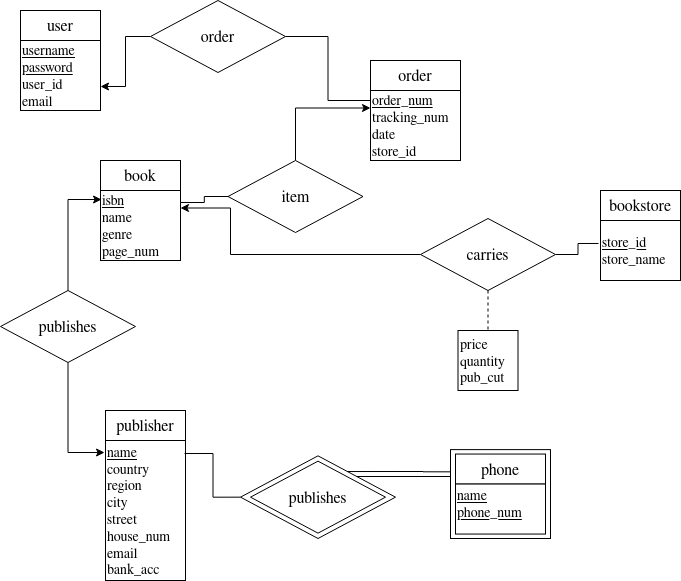
\includegraphics[scale=.65]{images/ERDiagram.png}
            \end{center}
        \subsection{Description}
        \subsection{Notes}
            \begin{itemize}
                \item The project description states ``When checkingout,  the user inserts billing and shipping information (can be different than those used in registration)''.
                This implies that billing and shipping should be inputted upon registration. I chose not to implement this because it poses an unnecessary security risk for users who have never made an order.
            \end{itemize}
    \section{Reduction to Relation Schema}
    \section{Normalization of Relation Schema}
    \section{Database Schema Diagram}
        \begin{center}
            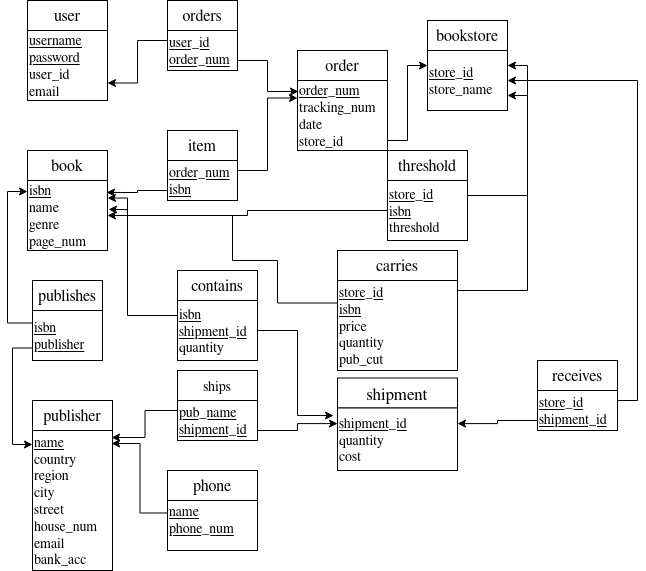
\includegraphics[scale=.7]{images/SchemaDiagram.png}
        \end{center}
    \section{Implementation}
    \section{Bonus Features}
    \section{GitHub Repo}
        Repository will be made public April 14. \\
        \url{https://github.com/AdamPayzant/COMP3005_Project}
\end{document}